\section{Experiments}
\label{sec:experiments}


\subsection{Statistical Framework}
\label{sec:stat_framework}

The primary family comprises six tests---three target judges (GPT-4o, Qwen3-32B, Llama-3.3-70B) $\times$ two axes (formality, verbosity)---corrected via Holm-Bonferroni at $\alpha = 0.05$; Gemini-2.5-Flash serves as confirmatory replication and is excluded from FWER control; as a sensitivity check, all eight tests remain significant under the expanded family (Appendix~\ref{app:holm8}).
Table~\ref{tab:main_results} reports both raw and adjusted $p$-values.
Analyses outside this grid are classified as either \emph{exploratory} (NLI threshold sensitivity sweep, \S\ref{sec:nli_threshold}) or \emph{confirmatory} (consistency filter validation, \S\ref{sec:consistency}).
Exploratory analyses use uncorrected $p$-values; confirmatory analyses (pipeline validity) are evaluated at $\alpha = 0.05$ without additional correction.
Bradley-Terry parameters \citep{bradley1952rank,luce1959individual} are estimated via spectral initialization followed by minorization-maximization \citep{hunter2004mm}, using the \texttt{choix} Python library's default L2 regularization ($\alpha = 10^{-6}$).
In binary-choice BT models, IIA is structurally satisfied; the direction asymmetry in Appendix~\ref{app:bt_gof} (formality: formal-origin 88.9\% vs.\ casual-origin 52.6\%, Fisher $p = 0.015$) reflects heterogeneous treatment effects rather than IIA violation.
All bootstrap confidence intervals are percentile CIs from 10{,}000 pair-level resamples with seed 42; we verify bootstrap stability by confirming that halving the resample count changes interval widths by $<$1pp.
GEE models use exchangeable working correlation with sandwich standard errors (robust to correlation misspecification), justified by near-zero estimated within-pair correlations ($\hat{\alpha} \in [-0.25, +0.11]$; Appendix~\ref{app:gee_diagnostics}).
A prospective power analysis (Appendix~\ref{app:power}) confirms that our sample sizes ($n = 86$--$88$ pairs) provide $>$90\% power to detect BT effects of the observed magnitude ($P \geq 0.63$), whereas Likert requires $4$--$206\times$ the sample size for equivalent power (Figure~\ref{fig:power_curve}).

\paragraph{Model selection.}
Target judges span four architectures from independent providers: GPT-4o (\texttt{2024-08-06}; OpenAI), Qwen3-32B-Instruct (Alibaba; also serving as rewriter), Llama-3.3-70B-Instruct (Meta), and Gemini-2.5-Flash (Google).
This diversity guards against provider-specific artifacts in both training data and RLHF reward modeling; Claude Sonnet~4 (Anthropic) provides discriminative validity evidence (\S\ref{sec:cross_judge}), serving as a fifth judge from a provider not represented in the primary family.
All judges are accessed via their respective APIs with temperature 0 (deterministic decoding) and default system prompts to ensure reproducibility.

\begin{table}[t]
\centering
\small
\caption{Primary results on LLMBar ($n = 88$ formality, $86$ verbosity, except where noted) across five judges and three style axes. BT $> 0.50$ indicates style preference; $\dagger$ marks Blindspot cases (BT significant, Likert not). Cross-benchmark replication in Appendix~\ref{app:cross_bench}. BT: Bradley-Terry win probability (95\% CIs in Appendix~\ref{app:bt_ci}).}
\label{tab:main_results}
\begin{tabular}{@{}llccc@{}}
\toprule
Judge & Axis & BT $P$ & Likert $d$ ($p$) & Cat.\ \\
\midrule
GPT-4o & Form.\ & .630$^{***}$ & $-$.041 (.905) & $\dagger$ \\
GPT-4o & Verb.\ & .760$^{***}$ & .049 (.403) & $\dagger$ \\
GPT-4o & Reg.\ & .570$^{\dagger}$ & .000 (.785) & $\dagger_{\text{e}}$ \\
\cmidrule{1-5}
Qwen3 & Form.\ & .665$^{***}$ & $-$.052 (.461) & $\dagger$ \\
Qwen3 & Form.$^b$ & .675$^{***}$ & $-$.025 (.600) & $\dagger$ \\
Qwen3 & Verb.\ & .773$^{***}$ & .036 (.395) & $\dagger$ \\
Qwen3 & Reg.\ & .553 & $-$.073 (.373) & $\dagger_{\text{e}}$ \\
\cmidrule{1-5}
Llama-70B & Form.\ & .695$^{***}$ & .010 (.534) & $\dagger$ \\
Llama-70B & Verb.\ & .735$^{***}$ & .020 (.284) & $\dagger$ \\
Llama-70B & Reg.\ & .635$^{\dagger}$ & .024 (.524) & $\dagger_{\text{e}}$ \\
\cmidrule{1-5}
Gemini & Form.\ & .574$^{*}$ & $-$.082 (.309) & $\dagger_{\text{c}}$ \\
Gemini & Verb.\ & .708$^{***}$ & .051 (.370) & $\dagger_{\text{c}}$ \\
\cmidrule{1-5}
Claude & Form.\ & .562 & $-$.021 (.721) & --- \\
Claude & Verb.\ & .541 & $-$.039 (.743) & --- \\
\bottomrule
\multicolumn{5}{@{}p{\columnwidth}@{}}{\footnotesize $^{***}\!p < 0.001$; $^{*}\!p < 0.05$ (Holm-adj.\ for primary; raw for $_{\text{c}}$). $\dagger$: Blindspot (BT sig., Likert n.s.); ---: neither sig.; $_{\text{e}}$: exploratory; $_{\text{c}}$: confirmatory. Negative $d$: styled variants scored lower.}\\
\multicolumn{5}{@{}p{\columnwidth}@{}}{\footnotesize $^b$ Scaled replication ($n = 355$). Qwen3 serves as both rewriter and judge; independent GPT-4o rewriter yields 22\% lower Style OR (App.~\ref{app:rewriter_indep}).}\\
\multicolumn{5}{@{}p{\columnwidth}@{}}{\footnotesize Form.\ direction asymmetry: formal-origin 78.8\% vs.\ casual-origin 54.5\%; GEE-adj.\ Style OR$=$2.58 ($p{=}.002$; App.~\ref{app:direction}).}
\end{tabular}
\end{table}


\begin{figure}[t]
\centering
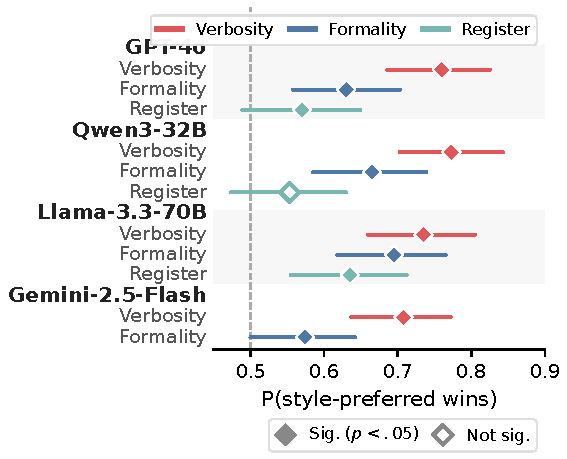
\includegraphics[width=\columnwidth]{figures/forest_plot.pdf}
\caption{Bradley-Terry win probabilities across four target judges and three style axes. Filled diamonds: significant ($p < 0.05$); open diamonds: non-significant. Error bars: 95\% bootstrap CI. The dashed line at 0.50 indicates no style preference. Verbosity shows the strongest and most consistent bias across all four judges.}
\label{fig:forest_plot}
\end{figure}

\section{Analysis}
\label{sec:analysis}


\subsection{The Likert Blindspot}
\label{sec:likert_pairwise}

\paragraph{Head-to-head comparison with RATE.}
Applying RATE's Likert ATE methodology \citep{reber2025rate} to our formality style-transformed pairs yields Cohen's $d = {-}0.04$, $p = 0.91$ (non-significant, $n = 88$); pairwise comparison on identical data reveals a 63.0\% formal preference ($p = 0.0004$, Bradley-Terry on all 173 comparisons), confirmed by a consistency-filtered sign test (73.9\%, $p = 0.006$, $n = 46$ consistent pairs).
This is the Likert Blindspot: the same data, the same style intervention, two measurement instruments---one detects bias, the other does not.
A $4\times$ scaled replication ($n = 355$) distinguishes measurement attenuation from insufficient power: the Likert effect size shrinks to $d = {-}0.025$ (near zero) while BT remains stable at $67.5\%$ ($p < 0.0001$)---if the gap were merely statistical power, $d$ would remain non-zero at larger $n$.
Bootstrap subsampling confirms $d$ remains near zero as $n$ grows (Appendix~\ref{app:bootstrap_attenuation}).
Post hoc, attenuation follows a severity spectrum: complete at moderate bias ($d \to 0$, BT 63--67\%) and partial at stronger effects (${>}60\%$ loss, BT ${>}70\%$)---explaining three cross-benchmark exceptions ($\ddagger$, Table~\ref{tab:cross_bench}).

RATE and CSD are complementary (Likert ATE vs.\ forced-choice BT); the Blindspot arises from Likert tie rates of 58--73\%, unresolved by 100-point continuous scaling (all three judges $p > 0.15$; Appendix~\ref{app:likert100}).


\paragraph{Sensitivity hierarchy across measurement methods.}
Seven measurement methods applied to the same formality data confirm the Blindspot is not test-specific: both pairwise methods detect the formality preference while all five Likert-based methods fail regardless of scaling assumption---interval (ATE $t$-test), ordinal (proportional odds), or nonparametric (Wilcoxon)---with verbosity showing the same pattern (Table~\ref{tab:sensitivity}, Appendix~\ref{app:sensitivity}; verbosity replication in Appendix~\ref{app:verb_sensitivity}).

Figure~\ref{fig:power_curve} plots detection probability at observed effect magnitudes (not post-hoc power; cf.\ \citealt{hoenig2001abuse}): across six cells, Likert requires $4$--$206\times$ the current $n$ ($336$--$27{,}159$ pairs; Appendix~\ref{app:power_analysis}) to detect effects BT identifies at $p < 0.001$ with $n \leq 100$.
Under format equivalence, observing 8/8 primary cells as Blindspot has binomial probability $p = 0.004$; non-tie concordance (76.6\%, $p < .001$; \S\ref{sec:likert_pairwise}) provides a complementary formal test of format divergence.
\paragraph{Interpreting the divergence.}
The measurement-mode divergence admits three non-exclusive interpretations: (a)~\emph{Likert attenuation}---tie inflation and residual signal loss reduce Likert sensitivity below detection thresholds; (b)~\emph{pairwise amplification}---forced-choice comparison inflates micro-preferences into apparent biases \citep{jeong2025comparative}; (c)~\emph{construct divergence}---the two formats measure different constructs (absolute quality vs.\ ordinal preference; \citealt{tripathi2025pairwise}).
Six experimental controls (\S\ref{sec:amplification}) bound the amplification factor but cannot eliminate it; the attenuation evidence ($d \to 0$ at $n = 355$) is necessary but not sufficient for causal identification.
Non-tie concordance analysis partially adjudicates: among 201 Likert non-tie pairs (pooled across judges and axes), 76.6\% agree with pairwise direction [70.3\%, 81.9\%], $p < 0.001$; point-biserial correlations are uniformly positive ($r = 0.20$--$0.45$, 7/9 significant; Appendix~\ref{app:concordance})---evidence more consistent with measurement attenuation than construct divergence, though partial construct divergence remains at weaker effect sizes.
Claude's benchmark-dependent profile illustrates why aggregate BT is insufficient for bias attribution: LLMBar formality shows near-null sensitivity (Style OR n.s.) while AEval verbosity reveals significant sensitivity (Style OR $= 4.76$, $p < .001$)---a pattern disambiguated only by per-axis GEE decomposition (\S\ref{sec:cross_judge}; Appendix~\ref{app:claude_tost}).
All three interpretations converge on one practical conclusion: single-format audits risk incomplete bias coverage; the Blindspot manifests in 8/11 bias-positive cells, with three exceptions ($\ddagger$) confirming effect-size dependence.
This finding has direct implications for alignment pipelines that use Likert-based reward models: biases embedded in reward signals may go undetected during model development, propagating style preferences into downstream model behavior without any diagnostic signal at standard evaluation scales.

\begin{figure}[t]
\centering
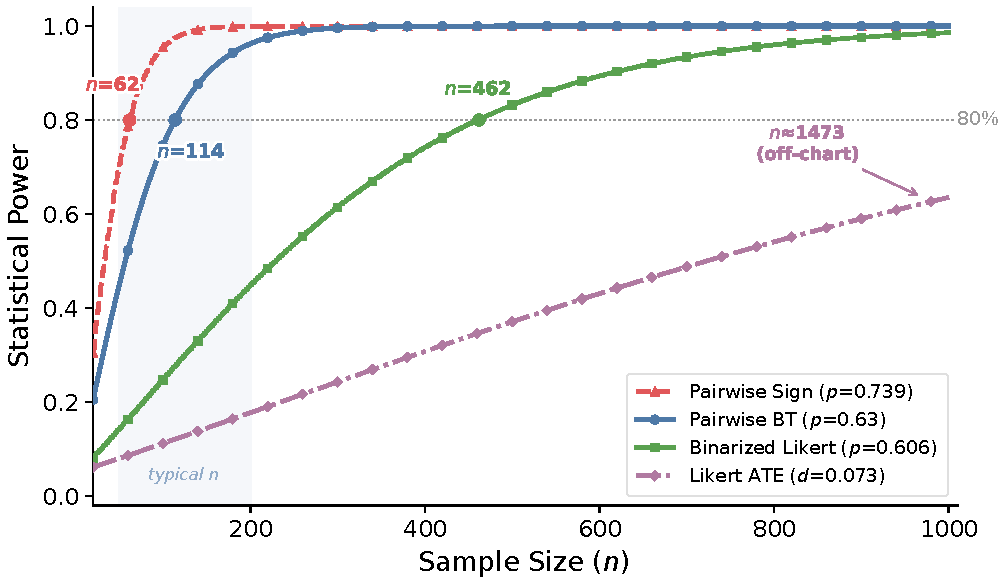
\includegraphics[width=\columnwidth]{figures/power_curve.pdf}
\caption{Detection probability at observed effect magnitudes. 80\% power crossings: sign test $n \approx 62$, BT $n \approx 114$, binarized Likert $n \approx 462$, Likert ATE $n \approx 1{,}473$. At typical scales ($n = 50$--$200$, shaded), pairwise methods reach 80\% power while Likert methods remain far below. At $n = 355$, Likert $d = {-}0.025$ confirms the gap is structural, not merely a power issue.}
\label{fig:power_curve}
\end{figure}

\subsection{Per-Axis Confound Structure}
\label{sec:direction}

GEE conditional decomposition \citep{liang1986gee} with exchangeable working correlation and robust standard errors separates style from originality effects (Appendix~\ref{app:direction}; model diagnostics including correlation structure robustness and interaction tests in Appendix~\ref{app:gee_diagnostics}).
After controlling for original preference, the formality effect remains significant (GPT-4o: OR $= 2.58$, $p = 0.002$; Qwen3-32B: OR $= 2.15$, $p < 0.0001$, $n = 355$; Llama-70B: OR $= 4.81$, $p < 0.0001$; Table~\ref{tab:gee}); the significant originality ORs confirm residual confounding.
For formality, both style preference and quality correlation contribute (a conditional effect); the two-predictor GEE provides a parsimonious decomposition rather than causal identification---omitted variables (text length, lexical complexity) may partly confound both terms.
This per-axis heterogeneity has direct implications for bias mitigation: verbosity bias can be addressed by style-level interventions (e.g., length normalization or debiased prompting), whereas formality bias requires disentangling genuine quality correlates from surface-level preferences---a fundamentally harder problem that aggregate bias metrics cannot even detect.

\begin{table}[t]
\centering
\small
\caption{GEE conditional decomposition (exchangeable correlation). Style OR: style-direction odds ratio; Orig OR: original-preference odds ratio (OR $> 1$ favors original). $n{=}88$ ORs are upper-bound estimates; scaled replications ($n = 330$--$355$) show $49$--$72\%$ shrinkage \citep{nemes2009bias}. Verbosity is style-dominated; formality shows varying confound structure.}
\label{tab:gee}
\begin{tabular}{@{}llclc@{}}
\toprule
 & \multicolumn{2}{c}{Style OR} & \multicolumn{2}{c}{Originality OR} \\
\cmidrule(lr){2-3} \cmidrule(lr){4-5}
Config & OR & $p$ & OR & $p$ \\
\midrule
Qwen3 verb.\ & 13.10 & ${<}.0001$ & 0.49 & .096 \\
GPT-4o verb.\ & 11.34 & ${<}.0001$ & 0.45 & .062 \\
Llama-70B verb.\ & 8.21 & ${<}.0001$ & 0.38 & .020 \\
Gemini verb.\ & 8.98 & ${<}.0001$ & 0.46 & .061 \\
\midrule
GPT-4o form.\ & 2.58 & .002 & 2.32 & .006 \\
Qwen3 form.\ & 4.20 & .0002 & 4.70 & .0001 \\
Qwen3 form.$^a$ & 2.15 & ${<}.0001$ & 4.99 & ${<}.0001$ \\
Llama-70B form.\ & 4.81 & ${<}.0001$ & 3.12 & .0007 \\
Gemini form.\ & 1.64 & .101 & 2.51 & .002 \\
\midrule
GPT-4o reg.\ & 1.88 & .029 & 2.21 & .006 \\
Qwen3 reg.\ & 1.91 & .046 & 5.72 & ${<}.0001$ \\
Llama-70B reg.\ & 3.33 & .0003 & 3.07 & .0008 \\
\bottomrule
\multicolumn{5}{l}{\footnotesize $^a$ $n = 355$; other rows: $n = 88$. 95\% CIs in Appendix.}
\end{tabular}
\end{table}

The confound structure is consistent across all four target judges for verbosity (style-dominated at $n = 88$: Style OR $8.2$--$13.1$, Orig OR $0.38$--$0.49$; confirmed at $n = 330$: Style OR $2.5$--$4.0$); formality is conditionally style-driven in three judges but originality-dominated in Gemini; register is judge-dependent (Figure~\ref{fig:gee_decomp}).
Same-style double-rewrite controls confirm a rewriting artifact (Appendix~\ref{app:artifact_control}), absorbed by GEE's originality term.

\begin{figure}[t]
\centering
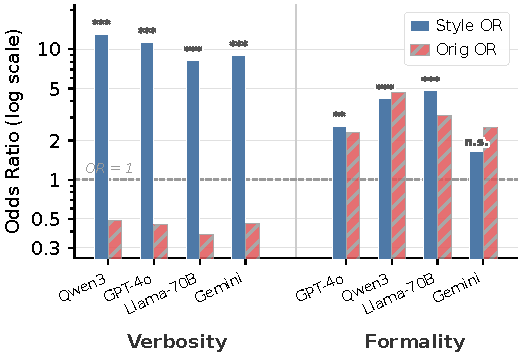
\includegraphics[width=\columnwidth]{figures/gee_decomposition.pdf}
\caption{GEE conditional decomposition across four judges ($n = 88$, LLMBar). Verbosity (left) is style-dominated: Style OR $\gg 1$, Originality OR $< 1$. Formality (right) shows joint contributions from both predictors. Dashed line: OR $= 1$ (no effect). Hatched bars: Originality OR. Log scale.}
\label{fig:gee_decomp}
\end{figure}

\paragraph{Sample-size sensitivity.}
At $n = 355$, the Qwen3-32B formality Style OR drops from $4.20$ to $2.15$ ($-49\%$), consistent with small-sample upward bias \citep{nemes2009bias}; the regime classification remains stable (both effects significant; Orig OR $4.70 \to 4.99$).
Verbosity $n = 330$ confirms 51--72\% GEE shrinkage (Style OR $2.5$--$4.0$; Appendix~\ref{app:verb_n355}), preserving the style-dominated classification; Likert begins detecting the strongest effects at this $n$, reframing the Blindspot as a $3$--$4\times$ efficiency gap rather than absolute failure.
This convergence at larger $n$ is practically important: it means that labs with sufficient evaluation budgets ($n > 300$) can detect the strongest biases with Likert alone, but typical benchmark sizes ($n = 50$--$200$) systematically miss them.

\subsection{Cross-Judge and Cross-Axis Replication}
\label{sec:cross_judge}

Two independent judges replicate the formality Blindspot: Qwen3-32B (BT 66.5\%, $p < 0.0001$; Likert $p = 0.461$) and Llama-3.3-70B (BT 69.5\%, $p = 0.0001$; Likert $p = 0.534$).
Gemini-2.5-Flash shows a weaker, originality-dominated formality pattern (confirmatory: BT 57.4\%, $p = 0.031$; Likert $d = {-}0.08$, n.s.; Style OR $= 1.64$, n.s.; Orig OR $= 2.51$, $p = 0.002$; \S\ref{sec:direction}).

Verbosity provides the strongest Blindspot: all four target judges show consistent preference (GPT-4o 76.0\%, Qwen3-32B 77.3\%, Llama-70B 73.5\%, Gemini 70.8\%; all $p \leq 0.0001$), while Likert ATE remains non-significant for all ($p = 0.284$--$0.403$).
GEE confirms style dominance (Style OR $8.2$--$13.1$, all $p < .0001$; Orig OR $0.38$--$0.49$; Table~\ref{tab:gee}).
Both rewriting directions favor verbose responses (90.7\%/80.6\%); length-controlled Style OR is unchanged ($<$2\%), and an independent GPT-4o rewriter bounds evaluator-producer overlap to a 22\% reduction (Appendix~\ref{app:rewriter_indep}).
Length-controlled regression confirms 60\% of the FK cross-axis effect is mediated by sentence length (Sobel $z = 2.15$, $p = .031$); under the assumed causal structure (Figure~\ref{fig:dag}), FK acts as a plausible mediator ($S \to \text{FK} \to Y$; \citealp{pearl2009causality}), yielding a direct-effect Style OR of $2.15$ for GPT-4o (total OR $= 2.70$; Appendix~\ref{app:fk_length}).

These per-axis patterns selectively replicate across benchmarks (6/24 possible cells; Figure~\ref{fig:cross_bench_heatmap}), targeting the strongest effects: Llama-70B formality on AlpacaEval (BT 75.0\%, Style OR $= 7.64$) is strong enough for Likert detection ($\ddagger$ rows), confirming the severity spectrum.
The selective replication strategy prioritizes cells where effects are strongest, providing an informative lower bound on cross-benchmark generalization without requiring exhaustive evaluation of all judge--axis--benchmark combinations.
Claude Sonnet~4 provides discriminative validity: near-null sensitivity on LLMBar (formality BT $= 0.562$, n.s.) but significant verbosity sensitivity on AlpacaEval (Style OR $= 4.76$, $p < .001$), demonstrating that CSD does not uniformly inflate bias estimates and that sensitivity profiles are benchmark-contingent even within a single judge.

\begin{figure}[t]
\centering
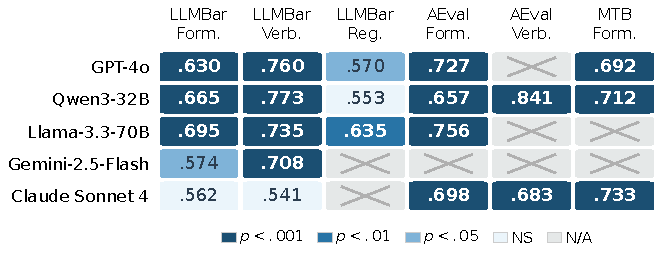
\includegraphics[width=\columnwidth]{figures/cross_benchmark_heatmap.pdf}
\caption{Pairwise BT win probabilities across five judges, three benchmarks, and three style axes. Bold: $p < .05$; color intensity encodes significance level. Grey $\times$: not tested. Claude cross-benchmark effects are quality-driven (\S\ref{sec:cross_judge}; Appendix~\ref{app:claude_crossbench}). Full results in Table~\ref{tab:cross_bench}.}
\label{fig:cross_bench_heatmap}
\end{figure}

\subsection{Robustness}
\label{sec:nli_validation}

\paragraph{Content preservation.}
Two independent annotators evaluated 100 NLI-scored pairs (50 per axis; 70 gate-passed, 30 gate-failed), confirming $98.6\%$ gate pass precision ($69/70$; AC$_1 = 0.96$; Appendix~\ref{app:annotation_agreement}).
\label{sec:nli_threshold}
BT remains stable (${\leq}3$pp variation) across 11 NLI thresholds (Appendix~\ref{app:nli_sweep}), confirming that results are not artifacts of a particular gating stringency.
Annotators judged only 49--66\% of NLI-passed pairs as showing detectable style change, suggesting observed effects represent a diluted lower bound on true style sensitivity---the NLI gate retains pairs with subtle rewrites that human annotators cannot detect, yet judges still systematically prefer one variant.

\paragraph{Detection vs.\ amplification.}
\label{sec:amplification}
\citet{jeong2025comparative} show that pairwise comparison amplifies style biases (the Comparative Trap).
The divergence cannot be definitively resolved without human ground-truth measurements; six controls bound amplification risk: (i)~NLI ablation reverses NLI-fail pairs (BT 41.7\%); (ii)~Claude shows benchmark-dependent sensitivity (formality Style OR n.s.; AEval verbosity OR $= 4.76$, $p < .001$); (iii)~cross-axis BT variation inconsistent with uniform amplification; (iv)~rewriting artifact absorbed by GEE; (v)~debiased prompting ($-5.2$/$-13.1$pp), bounding the amplification factor at ${\sim}9$--$17\%$ of the total BT effect; (vi)~four-architecture replication with consistent GEE structure.
Register is exploratory with evaluator-producer overlap and judge-dependent effects (Table~\ref{tab:gee}).
The combination of NLI validation and amplification controls establishes that while the exact magnitude of style sensitivity remains bounded rather than point-identified, the qualitative finding---systematic style preferences invisible to Likert---is robust across judges, axes, and measurement assumptions.
